\chapter{Калибровочные поля, масштабы взаимодействия и заряженные слабые токи}

Квантовая электродинамика и квантовая хромодинамика в лаборатории выглядят очень по-разному, однако обе являются калибровочными теориями. Более того, почти каждое взаимодействие в стандартной модели устроено именно так. Слово \emph{gauge} имеет более глубокий смысл, связанный с локальной симметрией, но этот аппарат мы пока можем отложить. Сейчас нам нужно минимальное физическое описание: калибровочная теория содержит поля, подобные максвелловским, сохраняющиеся источники, преобразования симметрии, калибровочные бозоны и правила испускания и поглощения этих бозонов.

\section{Теория Максвелла как прототип}

\subsection{Поля и потенциалы}

Электромагнитное поле имеет шесть компонент: три компоненты электрического поля и три компоненты магнитного поля. Та же информация, с некоторой избыточностью, может быть закодирована в четырёхвекторном потенциале
\begin{equation}
A_\mu=(A_0,\boldsymbol A),
\end{equation}
где \(A_0\) — электростатический потенциал, а \(\boldsymbol A\) — пространственный векторный потенциал. В электростатическом пределе электрическое поле получается из пространственного градиента,
\begin{equation}
\boldsymbol E=-\boldsymbol\nabla A_0,
\qquad
\boldsymbol F=q\boldsymbol E,
\end{equation}
тогда как магнитное поле равно
\begin{equation}
\boldsymbol B=\boldsymbol\nabla\times\boldsymbol A.
\end{equation}
Знак в первом уравнении зависит от принятого стандартного определения потенциала; обсуждение у доски в основном касается того факта, что поля являются производными потенциалов.
\editorialnote{Для зависящих от времени полей полное соотношение имеет вид
\(\boldsymbol E=-\boldsymbol\nabla A_0-\partial_t\boldsymbol A\). Здесь в лекции намеренно рассматривается более простой электростатический уровень.}

\begin{figure}[htbp]
\centering
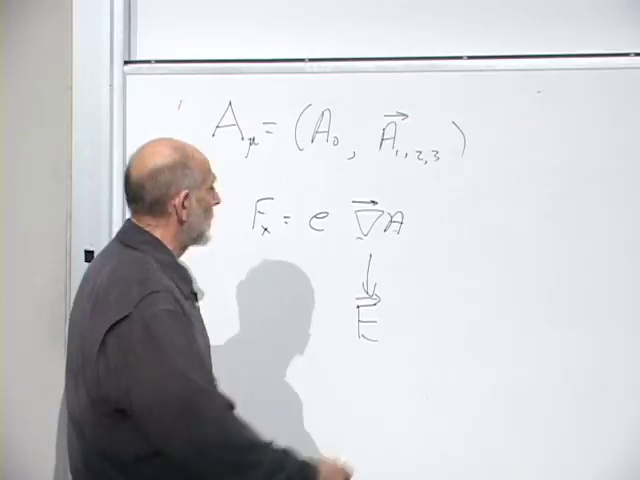
\includegraphics[width=0.62\textwidth]{lecture_05_figure_02.png}
\caption{Электромагнитный четырёхпотенциал и его связь с полем через производные.}
\lectureframe{00:03:33}
\end{figure}

Таким образом, электродинамика допускает два эквивалентных описания: одно через \(\boldsymbol E\) и \(\boldsymbol B\), а другое через \(A_\mu\). Во втором явно выписаны только четыре компоненты, потому что одни и те же физические поля могут описываться разными потенциалами. Эта избыточность — первый намёк на смысл слова калибровка, хотя формально мы этим пока пользоваться не будем.

\subsection{Волны и поляризация}

Уравнения Максвелла допускают волны. Рассмотрим плоскую волну, распространяющуюся вдоль единичного вектора \(\hat{\boldsymbol k}\). В каждой точке электрическое и магнитное поля поперечны:
\begin{equation}
\boldsymbol E\cdot\hat{\boldsymbol k}=0,
\qquad
\boldsymbol B\cdot\hat{\boldsymbol k}=0,
\qquad
\boldsymbol E\cdot\boldsymbol B=0.
\end{equation}
В единицах, где \(c=1\), их модули равны,
\begin{equation}
|\boldsymbol E|=|\boldsymbol B|.
\end{equation}
Для линейно поляризованной волны направление \(\boldsymbol E\) задаёт поляризацию. Вся конфигурация распространяется со скоростью света.

Квантование меняет язык описания, но не структуру поляризации. Квант электромагнитной волны — это фотон. Изображать фотон точкой неизбежно вводит в заблуждение, но полезно вообразить, что эта точка несёт маленькую поперечную стрелку, фиксирующую его поляризацию. Четвертьволновая пластинка или другой оптический элемент может поворачивать её. Статическое кулоновское поле аналогичным образом тоже можно, хотя лишь грубо, представлять как возникающее из многократного испускания и поглощения фотонов.

\subsection{Источники, поток и сохранение}

Электромагнитные волны могут распространяться в пустом пространстве, но у поля есть и источники: электрические заряды и токи. Положительный точечный заряд создаёт направленное наружу радиальное электрическое поле, пропорциональное \(1/r^2\). Число силовых линий, проходящих через любую сферу вокруг заряда, не зависит от радиуса этой сферы. Математически,
\begin{equation}
\oint_{S^2}\boldsymbol E\cdot d\boldsymbol S
=\frac{Q_{\mathrm{enc}}}{\epsilon_0},
\label{eq:l5-gauss}
\end{equation}
в единицах СИ.

Это больше, чем просто удобный способ вычислять поле. Линии электрического поля могут оканчиваться только на заряде. Если бы один изолированный заряд просто исчез, его поле либо должно было бы исчезнуть сразу повсюду, нарушая причинность, либо наружу должен был бы распространяться фронт исчезнувшего поля, причём силовые линии оканчивались бы в пустом пространстве. Ни то ни другое недопустимо. Поэтому геометрия потока делает сохранение заряда естественным: заряд может перемещаться, противоположные заряды могут аннигилировать, но суммарный заряд не может локально исчезнуть без компенсирующего тока.

Соответствующее локальное утверждение — это уравнение непрерывности
\begin{equation}
\partial_t\rho+\boldsymbol\nabla\cdot\boldsymbol J=0.
\label{eq:l5-continuity}
\end{equation}
\editorialnote{Уравнение~\eqref{eq:l5-continuity} — это стандартная локальная математическая форма причинного аргумента о потоке, который в лекции излагался словами.}

\subsection{Рабочее определение калибровочной теории}

Теперь мы можем сформулировать рабочую схему. Калибровочная теория имеет:
\begin{itemize}
\item поля, подобные электрическому и магнитному;
\item волны, которые, если взаимодействия достаточно слабы, напоминают световые волны;
\item источники, аналогичные электрическому заряду;
\item закон Гаусса, связывающий поток с этими источниками;
\item закон сохранения и связанную с ним симметрию;
\item кванты поля, называемые калибровочными бозонами; и
\item константу связи, управляющую испусканием и поглощением.
\end{itemize}
Источник не обязан быть электрическим зарядом. В качестве заведомо нефизического примера представим, что барионное число сделано калибровочным. И протоны, и нейтроны имеют барионное число \(+1\), так что они отталкивались бы посредством новой кулоноподобной силы; протон и антипротон притягивались бы. Такую теорию можно вообразить математически, но в природе не наблюдается дальнодействующего калибровочного поля, связанного с барионным числом. Само по себе сохранение не гарантирует калибровочную силу.

У электрического заряда действительно есть соответствующая симметрия. Для заряженного поля вещества,
\begin{equation}
\psi(x)\longmapsto e^{i\theta}\psi(x).
\label{eq:l5-u1}
\end{equation}
Фазовая симметрия и сохранение заряда — две стороны одной и той же структуры. Позже мы сможем сделать \(\theta\) зависящей от пространства-времени и увидеть, почему требуется потенциал \(A_\mu\). Здесь глобального преобразования достаточно, чтобы выделить сохраняющийся заряд.

\section{Квантовая хромодинамика как неабелевский пример}

\subsection{Триплеты, антитриплеты и матрица глюонного поля}

В квантовой хромодинамике кварковое поле несёт цветовой индекс \(i\in\{r,g,b\}\) и преобразуется по фундаментальному представлению группы \(SU(3)\):
\begin{equation}
q'_i=U_{ij}q_j,
\qquad
U^\dagger U=\boldsymbol 1,
\qquad
\det U=1.
\label{eq:l5-q-transform}
\end{equation}
Это поворот в трёхмерном комплексном цветовом пространстве, а не поворот обычного координатного пространства. Трёхкомпонентное представление также называют определяющим представлением.

Поля античастиц представляются комплексно-сопряжёнными переменными. Комплексное сопряжение уравнения~\eqref{eq:l5-q-transform} даёт
\begin{equation}
q_i^{\prime *}=U_{ij}^*q_j^*.
\label{eq:l5-antiquark-transform}
\end{equation}
Таким образом, кварки преобразуются как \(\boldsymbol 3\), тогда как антикварки преобразуются как \(\bar{\boldsymbol 3}\).

\begin{figure}[htbp]
\centering
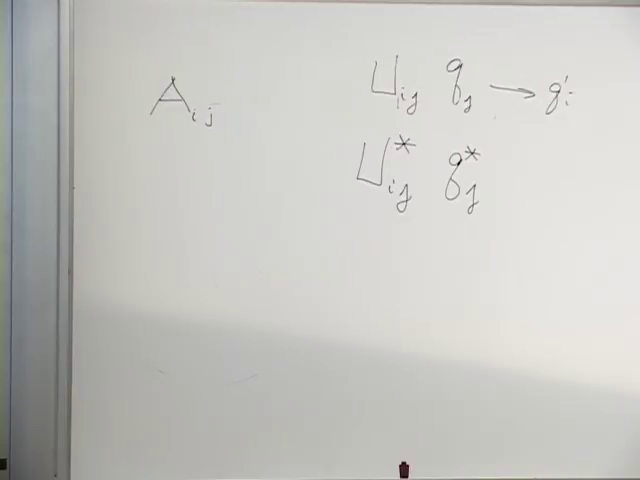
\includegraphics[width=0.62\textwidth]{lecture_05_figure_03.png}
\caption{Фундаментальное преобразование и его комплексно-сопряжённое антитриплетное преобразование.}
\lectureframe{00:18:47}
\end{figure}

\begin{classroomqa}
\audiencequestion{Сколько матриц \(U\) существует -- семь, восемь или девять?
\lecturetimestamp{00:19:37}}
\lecturerresponse{Элементов группы \(U\) бесконечно много. Подсчитываемое конечное число — это число независимых генераторов, и для \(SU(3)\) оно равно восьми. У общей матрицы \(3\times3\) девять позиций, но условие специальной унитарности оставляет восемь непрерывных направлений.}
\end{classroomqa}

Глюонное поле можно записать как матрицу \(A_{ij}\) со нулевым следом. Один индекс преобразуется как у кварка, а другой — как у антикварка, поэтому его цветовая структура имеет вид
\begin{equation}
\boldsymbol 3\otimes\bar{\boldsymbol 3}
=\boldsymbol 1\oplus\boldsymbol 8.
\end{equation}
В КХД сохраняется бесследовый октет,
\begin{equation}
A_{ii}=\operatorname{tr}A=0,
\end{equation}
а синглет отбрасывается. Поэтому в КХД восемь глюонов, а не девять. Более общо, группа \(SU(N)\) имеет
\begin{equation}
N^2-1
\end{equation}
генераторов и столько же полей калибровочных бозонов.

Фотон нейтрален относительно электрического \(U(1)\): поворот фазы электрона не превращает фотон в другой фотон. С глюонами иначе. Глюон несёт цвет и антицвет, поэтому он преобразуется по присоединённому представлению. Например, комбинация красный--антисиний не является цветовым синглетом, хотя в ней есть один цвет и один антицвет.

\subsection{Поток индексов и самовзаимодействие}

Правило взаимодействия можно прочитать, прослеживая индексы. Схематически кварк цвета \(i\) может стать кварком цвета \(j\), испустив глюон, несущий соответствующий поток цвета:
\begin{equation}
q_i\longrightarrow q_j+A_{ij}.
\label{eq:l5-quark-gluon-vertex}
\end{equation}
Точное расположение \(i\) и \(j\) зависит от соглашения о направлении стрелок; инвариантное содержание состоит в том, что каждый индекс, входящий в вершину, должен продолжиться по другой линии. Ни один цветовой индекс не теряется.

Это правило действует в любой калибровочной теории \(SU(N)\). Фундаментальная материя имеет один индекс, антифундаментальная материя имеет один сопряжённый индекс, а калибровочный бозон имеет по одному индексу каждого типа. Физические названия могут меняться, но индексная структура остаётся.

Поскольку глюон сам несёт цвет, он может испустить другой глюон. Глюон \(A_{ij}\) может расщепиться через промежуточный индекс \(k\); схематически,
\begin{equation}
A_{ij}\longrightarrow A_{ik}+A_{kj}.
\label{eq:l5-three-gluon-index}
\end{equation}
Это не полная вершина Янга--Миллса, но она показывает поток цвета. В обычной электродинамике для фотонов ничего аналогичного не происходит. Поэтому глюоны оказывают силовое воздействие друг на друга, и динамика неабелевых полей гораздо сложнее, чем линейная теория Максвелла.

Одно качественное следствие — конфайнмент. Линии потока цветового поля не могут обрываться, и их самодействие стягивает их в трубку, соединяющую кварк с антикварком. Эта трубка несет приблизительно постоянную энергию на единицу длины:
\begin{equation}
V(R)\simeq \sigma R.
\end{equation}
Поэтому, если раздвигать ее концы дальше, запасается все больше энергии, а не высвобождается изолированный цвет. Это и есть картина тягучего клея: само поле не позволяет цветным составляющим вырваться в виде свободных частиц.

\section{Константы связи и смысл слов сильный и слабый}

\subsection{Заряд как амплитуда испускания}

Калибровочной теории все равно нужна константа связи. В КЭД заряд электрона \(e\) — это коэффициент, связанный с вершиной электрон--фотон. Это амплитуда, а вероятности — квадраты амплитуд. Операционально можно представить, что быстрый электрон резко тормозится в электронно-лучевой трубке. Вероятность излучить фотон пропорциональна \(e^2\), причем стандартные множители поглощены в постоянную тонкой структуры,
\begin{equation}
\alpha=\frac{e^2}{4\pi\hbar c}
\simeq \frac{1}{137}.
\label{eq:l5-alpha}
\end{equation}
В естественных единицах \(\hbar=c=1\) константа связи безразмерна. Масштаб порядка одного процента для элементарного акта испускания делает электромагнетизм слабым в пертурбативном смысле: большинство остановленных электронов не испускают целый веер жестких фотонов.

\subsection{Естественные единицы связывают энергию, время и расстояние}

Положим
\begin{equation}
c=1,
\qquad
\hbar=1.
\end{equation}
Тогда время и расстояние имеют одни и те же единицы, а энергия — обратные единицы:
\begin{equation}
E=\hbar\omega\longrightarrow E=\omega\sim\frac1t,
\qquad
x\sim t\sim\frac1E.
\end{equation}
Большие энергии зондируют малые расстояния и короткие времена.

Для ориентировки,
\begin{equation}
1\ {\rm eV}^{-1}
=\frac{\hbar c}{1\ {\rm eV}}
\simeq 1.97\times10^{-7}\ {\rm m}.
\end{equation}
Поэтому атомный масштаб длины порядка \(10^{-10}\ {\rm m}\) приблизительно соответствует обратному килоэлектронвольту. Это пересчеты по порядку величины, а не точная спектроскопия.

\subsection{Иерархия внутри атома}

Для типичного атома возьмем
\begin{equation}
R_{\rm atom}\sim10^{-10}\ {\rm m}.
\end{equation}
Свет проходит это расстояние за
\begin{equation}
t_{\rm transit}^{\rm atom}\sim10^{-18}\ {\rm s}.
\end{equation}
Однако в легком атоме электрон движется лишь с малой долей скорости света. В боровской картине \(v/c\sim\alpha\), поэтому типичное орбитальное время больше:
\begin{equation}
t_{\rm orbit}^{\rm atom}\sim10^{-16}\ {\rm s}.
\end{equation}

Возбужденному атому требуется еще больше времени, чтобы излучить:
\begin{equation}
t_{\rm decay}^{\rm atom}\sim10^{-9}\ {\rm s}
\end{equation}
как грубая оценка на уровне лекции. В физической картине есть два подавляющих фактора. Электромагнитная сила создает лишь умеренное ускорение, а у ускоренного электрона есть еще одна малая вероятность испускания, определяемая \(\alpha\). Поэтому малая постоянная тонкой структуры создает иерархию между временами пролета, орбитального движения и радиационного распада.

\subsection{Отсутствие иерархии в адроне}

Адрон — это атомоподобная связанная система из кварков и глюонов, но ее масштаб гораздо меньше:
\begin{equation}
R_{\rm hadron}\sim10^{-15}\ {\rm m},
\qquad
t_{\rm transit}^{\rm hadron}\sim10^{-23}\ {\rm s}.
\end{equation}
Кварки пересекают адрон практически за то же время, и возбужденные адроны, распадающиеся сильным образом, тоже живут примерно
\begin{equation}
t_{\rm orbit}^{\rm hadron}
\sim t_{\rm decay}^{\rm hadron}
\sim10^{-23}\ {\rm s}.
\end{equation}
Адрон после удара может заколебаться и испустить пион почти настолько быстро, насколько это допускает причинность. Здесь нет разделения на семь или девять порядков величины, как внутри атома.

\begin{classroomqa}
\audiencequestion{Следует ли из специальной теории относительности, что адрон не может распадаться существенно быстрее, чем за время прохождения света через него?
\lecturetimestamp{00:47:15}}
\lecturerresponse{Так вполне корректно формулировать эту оценку по порядку величины. Сильные распады происходят примерно так быстро, как допускает размер системы; нет ни малой константы связи, ни другого большого подавления, которое их замедляло бы.}
\end{classroomqa}

Соответствующая сильная константа связи поэтому намного больше, чем \(\alpha\). На иллюстративном адронном масштабе в лекции приводится
\begin{equation}
\alpha_{\rm QCD}\sim0.2,
\end{equation}
что гораздо ближе к единице, чем \(1/137\). Таково динамическое происхождение более старого названия \emph{сильные взаимодействия}.
\editorialnote{Константа связи КХД зависит от энергии, поэтому \(\alpha_s\) не является одним фиксированным числом. Приведенное значение — иллюстративное зависящее от масштаба значение, как и подразумевается в лекции.}

\begin{classroomqa}
\audiencequestion{Называют ли сильный аналог просто константой сильного взаимодействия?
\lecturetimestamp{00:48:17}}
\lecturerresponse{По принятому соглашению ее называют \(\alpha_{\rm QCD}\) или, чаще, \(\alpha_s\). Электромагнитную обычно обозначают просто \(\alpha\), хотя \(\alpha_{\rm QED}\) можно использовать, когда обе появляются в одном и том же обсуждении.}
\end{classroomqa}

\begin{classroomqa}
\audiencequestion{Будет ли статья различать голую электромагнитную константу связи и измеренное, экранированное значение?
\lecturetimestamp{00:48:38}}
\lecturerresponse{Да. Говорят о голой константе связи и о перенормированной константе связи. Поляризация вакуума делает эффективную константу связи зависящей от масштаба, на котором она измеряется.}
\end{classroomqa}

\section{Загадка слабого распада}

Слабые взаимодействия получили свое название из-за связанных с ними очень больших времен распада. Обычно они медленнее сильных распадов и могут быть медленнее даже атомного излучения. Старейший пример — ядерный бета-распад.

\subsection{Нейтронный бета-распад}

Свободный нейтрон распадается по схеме
\begin{equation}
n\longrightarrow p+e^-+\bar\nu_e.
\label{eq:l5-neutron-decay-intro}
\end{equation}
На лекции используется время жизни порядка двенадцати минут, абсурдно большое по сравнению с \(10^{-23}\ {\rm s}\). Современные точные значения для этого рассуждения несущественны.

Часть этой медленности кинематическая. Грубо говоря,
\begin{equation}
\begin{aligned}
m_n&\simeq940\ {\rm MeV},
&
m_p&\simeq939\ {\rm MeV},
\\
m_e&\simeq0.5\ {\rm MeV}.
\end{aligned}
\end{equation}
Лишь ничтожная доля энергии покоя нейтрона доступна как кинетическая энергия. Если бы нейтрон был легче суммы конечных масс покоя, распад был бы невозможен. Если бы он находился лишь бесконечно мало выше порога, доступное фазовое пространство было бы крошечным, и распад был бы медленным. Но одно лишь фазовое пространство не может объяснить время жизни, измеряемое минутами.

\subsection{Заряженный пион устраняет оправдание порогом}

Рассмотрим также
\begin{equation}
\pi^-\longrightarrow e^-+\bar\nu_e
\end{equation}
и его зарядово-сопряженный процесс. У пиона имеется большой избыток энергии для электронного канала, однако его слабое время жизни все равно имеет порядок наносекунд, а не адронный порядок \(10^{-23}\) секунды. Сходный канал с мюоном вскоре станет важным. Следовательно, загадка присуща самому слабому взаимодействию, а не является просто случайностью почти вырожденных масс в нейтронном случае.

\editorialnote{Время жизни заряженного пиона составляет около \(26\ {\rm ns}\), а доминирующим каналом является \(\pi^-\to\mu^-\bar\nu_\mu\). Электронный канал подавлен по спиральности. На лекции сначала используется электронный канал, поскольку в нем проще всего вести учет частиц, а затем рассмотрение возвращается к доминирующему мюонному каналу.}

Термин бета-распад исторически возник из того, что испускаемые электроны называли бета-лучами. Примеры с пионом и нейтроном включают одно и то же взаимодействие заряженного тока, хотя их кинематика резко различается.

\section{Таблица кварков и лептонов}

\subsection{Цвет действует по вертикали}

Расположим шесть ароматов кварков в трех парных столбцах,
\begin{equation}
(u,d),\qquad(c,s),\qquad(t,b),
\end{equation}
и поместим красную, зеленую и синюю копию каждого кварка в отдельные строки. Цвет \(SU(3)\) действует по вертикали: он вращает друг в друга красную, зеленую и синюю версии u-кварка и одновременно выполняет то же цветовое вращение для d-, c-, s-, t- и b-кварков. Он не превращает u-кварк в d-кварк.

\subsection{Слабый изоспин действует по горизонтали}

Слабая симметрия действует в другом направлении. Она смешивает каждую соседнюю пару
\begin{equation}
Q_1=\begin{pmatrix}u\\d\end{pmatrix},
\qquad
Q_2=\begin{pmatrix}c\\s\end{pmatrix},
\qquad
Q_3=\begin{pmatrix}t\\b\end{pmatrix}.
\label{eq:l5-quark-doublets}
\end{equation}
У кварков верхнего типа заряд \(+2/3\), а у кварков нижнего типа заряд \(-1/3\), так что при переходе через каждую пару заряд меняется на единицу.
\editorialnote{В источнике на мгновение говорится, что d-кварк имеет заряд \(-2/3\). Вычитание в этом месте и все последующие процессы требуют стандартного значения \(-1/3\), которое и используется здесь.}

Поскольку симметрия действует на дублеты, естественной группой является \(SU(2)\). Она действует на каждую цветовую копию каждого кваркового дублета, не изменяя цвет.

Есть и четвертая строка частиц, не несущих цвет и потому не взаимодействующих с глюонами: лептоны. Они образуют еще три дублета,
\begin{equation}
L_e=\begin{pmatrix}\nu_e\\e^-\end{pmatrix},
\qquad
L_\mu=\begin{pmatrix}\nu_\mu\\\mu^-\end{pmatrix},
\qquad
L_\tau=\begin{pmatrix}\nu_\tau\\\tau^-\end{pmatrix}.
\label{eq:l5-lepton-doublets}
\end{equation}
Нейтрино электрически нейтральны; электрон, мюон и тау имеют заряд \(-1\). И здесь оба члена дублета различаются на одну единицу электрического заряда. Электрон, мюон и тау имеют одни и те же калибровочные квантовые числа, но разные массы, подобно тому как три поколения кварков верхнего или нижнего типа повторяют ту же схему зарядов.

\begin{figure}[htbp]
\centering
\includegraphics[width=0.82\textwidth]{lecture_05_figure_05.png}
\caption{Таблица на доске: цвет действует между красной, синей и зеленой строками, тогда как слабое \(SU(2)\) связывает попарно объединенные столбцы ароматов и лептонную строку.}
\lectureframe{01:03:35}
\end{figure}

Называть лептоны четвертым цветом — пока лишь аналогия. Они заполняют четвертую строку в таблице слабых дублетов, но обычная КХД \(SU(3)\) не преобразует кварки в лептоны.

\section{Построение заряженных слабых бозонов}

\subsection{Квантовые числа заряженных бозонов}

Калибровочные бозоны несут свойства преобразования, необходимые для перехода от одного члена дублета к другому. Начнём с лептонной пары
\(e^-\bar\nu_e\). Она имеет электрический заряд \(-1\), поэтому соответствующий заряженный калибровочный бозон называется \(W^-\):
\begin{equation}
W^-\sim e^-\bar\nu_e.
\end{equation}
Те же квантовые числа возникают у d-кварка и анти-u-кварка:
\begin{equation}
W^-\sim d\bar u.
\end{equation}
Символ \(\sim\) означает: имеет те же существенные калибровочные квантовые числа, что и.
Это не означает, что \(W\) буквально является связанным состоянием этих частиц.
Для античастицы получаются сопряжённые комбинации,
\begin{equation}
W^+\sim e^+\nu_e\sim\bar d u.
\end{equation}

Вершины заряженного слабого взаимодействия включают
\begin{align}
e^-&\longrightarrow\nu_e+W^-,
&
\mu^-&\longrightarrow\nu_\mu+W^-,
\label{eq:l5-lepton-w}\\
d&\longrightarrow u+W^-,
&
s&\longrightarrow c+W^-,
\label{eq:l5-quark-w}
\end{align}
с аналогичными переходами для третьего поколения, когда они кинематически разрешены. Калибровочный бозон динамически осуществляет то же горизонтальное смешивание, которое симметрия осуществляет в дублете.

\begin{classroomqa}
\audiencequestion{Сохранение заряда определяет, что испускаемый бозон должен иметь заряд
\(-1\), но почему переходы электрона, d-кварка и s-кварка
все должны включать одну и ту же частицу?
\lecturetimestamp{01:12:56}}
\lecturerresponse{Это эмпирический факт, закодированный общей слабой
симметрией. Природа могла бы непротиворечиво приписать отдельный бозон типа \(W\)
каждому семейству или кваркам и лептонам по отдельности. Вместо этого одно
\(SU(2)\) действует одновременно на все дублеты, и одни и те же заряженные калибровочные
бозоны опосредуют все эти переходы.}
\end{classroomqa}

\subsection{Чтение вершины и её обращение}

Одна вершина представляет целое семейство процессов. Если входящую линию
сделать исходящей, частица превращается в свою античастицу, а обращение линии
\(W^-\) даёт \(W^+\). Поэтому вершину можно читать как испускание,
поглощение, распад, аннигиляцию или обратную реакцию, если последовательно
соблюдать заряд, импульс и все существенные квантовые числа.

\begin{classroomqa}
\audiencequestion{Можно ли перевернуть стрелки и линии в этих слабых вершинах?
\lecturetimestamp{01:14:51}}
\lecturerresponse{Да. Линию можно перенести из конечного состояния в
начальное или наоборот, но тогда частица становится своей античастицей.
Поэтому одна и та же локальная вершина описывает много реакций с различной
ориентацией.}
\end{classroomqa}

\begin{classroomqa}
\audiencequestion{Означает ли запись \(W^-\) с линиями странного и очарованного
кварков, что этот бозон буквально является связанным состоянием странного кварка и
антиочарованного кварка?
\lecturetimestamp{01:15:43}}
\lecturerresponse{Нет. Учёт линий лишь говорит, что \(W^-\) несёт
изменение квантовых чисел между этими столбцами. Если читать диаграмму как
распад, достаточно энергичный \(W^-\) может породить странный кварк и
антиочарованный кварк; он не состоит из них.}
\end{classroomqa}

\begin{classroomqa}
\audiencequestion{Могут ли электрон и антинейтрино образовать \(W\), который затем
породит кварковую пару?
\lecturetimestamp{01:17:22}}
\lecturerresponse{Именно. Если доступна достаточная энергия в системе центра масс,
начальные лептоны могут образовать промежуточное состояние заряженного тока, и это состояние
может реализоваться в разрешённом кварковом канале. Эти две вершины — те же самые,
что используются в распаде, только прочитанные в другой ориентации.}
\end{classroomqa}

\subsection{Недостающий третий бозон}

Группа \(SU(2)\) имеет три генератора, а значит, три калибровочных поля. Пока что мы
явно показали только \(W^+\) и \(W^-\). Третье, электрически нейтральное поле
должно быть связано с диагональными комбинациями, такими как квантовые числа электрона--позитрона и
нейтрино--антинейтрино. Его намеренно оставляют скрытым на заднем
плане. Его связь с физическим бозоном \(Z\) и фотоном требует
электрослабого смешивания, к которому мы перейдём позже.

\begin{classroomqa}
\audiencequestion{Начали ли подозревать существование слабого и сильного взаимодействий в
разные исторические периоды?
\lecturetimestamp{01:24:11}}
\lecturerresponse{Их экспериментальные корни проявились вместе в ранних
исследованиях радиоактивности. Альфа-распад выявил ядерную физику и физику
сильного взаимодействия, бета-распад выявил слабое взаимодействие, а при
гамма-распаде испускались электромагнитные фотоны. В эпоху Беккереля уже
содержались все три указания, задолго до появления их современных полевых теорий.}
\end{classroomqa}

\section{Разобранные распады по заряженному току}

\subsection{Распад пиона}

Отрицательно заряженный пион имеет валентный кварковый состав
\begin{equation}
\pi^-=d\bar u.
\end{equation}
Эти квантовые числа могут аннигилировать в \(W^-\), который затем может породить
заряженный лептон и соответствующее антинейтрино:
\begin{align}
\pi^-&\longrightarrow W^{-*}
\longrightarrow e^-+\bar\nu_e,
\label{eq:l5-pion-electron}\\
\pi^-&\longrightarrow W^{-*}
\longrightarrow \mu^-+\bar\nu_\mu.
\label{eq:l5-pion-muon}
\end{align}
Звёздочка напоминает нам, что промежуточный \(W\) виртуален. Второй канал
является доминирующим.

\begin{figure}[htbp]
\centering
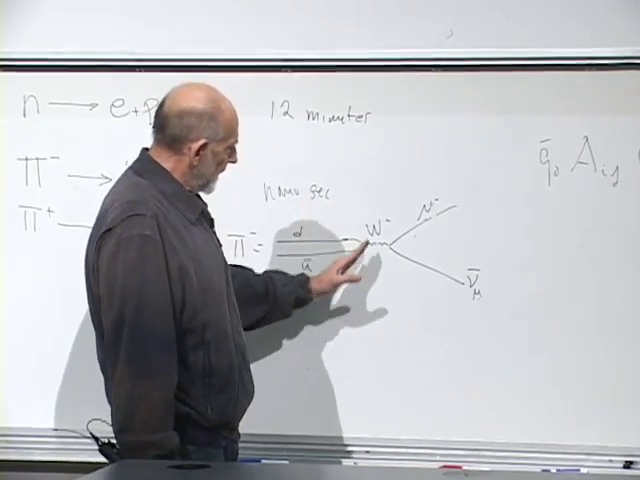
\includegraphics[width=0.72\textwidth]{lecture_05_figure_04.png}
\caption{Пион \(d\bar u\) аннигилирует в виртуальный \(W^-\), после чего
рождаются заряженный лептон и соответствующее ему антинейтрино.}
\lectureframe{01:19:38}
\end{figure}

\begin{classroomqa}
\audiencequestion{Действительно ли это диаграмма Фейнмана, хотя направление
времени нарисовано горизонтально, а не вертикально?
\lecturetimestamp{01:20:21}}
\lecturerresponse{Да. Ориентация времени на странице — дело соглашения.
Как только одно направление объявлено временем и все стрелки интерпретируются
последовательно, рисунок несёт ту же информацию о взаимодействии.}
\end{classroomqa}

\begin{classroomqa}
\audiencequestion{Можно ли читать эту диаграмму скорее как обратимую химическую
реакцию, а не как необратимый односторонний распад?
\lecturetimestamp{01:21:35}}
\lecturerresponse{Обратный процесс разрешён. Пион, возникший в пустом
пространстве, распадается, потому что вылетающие частицы разлетаются и обычно
не рекомбинируют. Но если мюон и антинейтрино направить навстречу друг другу с подходящими
энергией и импульсом, существует ненулевая амплитуда образования пиона через
обратное взаимодействие.}
\end{classroomqa}

\subsection{Энергия и виртуальное промежуточное состояние}

Для покоящегося пиона,
\begin{equation}
m_\pi\simeq140\ {\rm MeV},
\qquad
m_\mu\simeq106\ {\rm MeV},
\qquad
m_\nu\approx0
\end{equation}
с точностью, существенной здесь. Оставшаяся энергия переходит в кинетическую энергию
вылетающих частиц. Сохранение импульса требует
\begin{equation}
\boldsymbol p_\mu+\boldsymbol p_{\bar\nu}=0,
\end{equation}
так что в системе покоя пиона две частицы разлетаются в противоположных направлениях.

\begin{classroomqa}
\audiencequestion{Как может сохраняться энергия, если промежуточный \(W\)
намного тяжелее пиона?
\lecturetimestamp{01:25:08}}
\lecturerresponse{Только начальные и конечные частицы обязаны быть на массовой
оболочке. Четырёхимпульс сохраняется в каждой вершине, но внутренняя виртуальная
линия не обязана удовлетворять \(E^2=\boldsymbol p^2+m_W^2\). Чем больше её отклонение
от массовой оболочки, тем сильнее её пропагатор подавляет процесс.\editorialnote{В лекции используется традиционный язык соотношения неопределённостей
энергия--время и говорится, что промежуточное состояние может кратковременно нарушать сохранение энергии. Современная точная формулировка дана в ответе: энергия-импульс сохраняется, тогда как виртуальная внутренняя линия не обязана удовлетворять условию массовой оболочки для реальной частицы.}}
\end{classroomqa}

\subsection{Распад мюона}

Мюон может сначала перейти в своё нейтрино, испустив виртуальный \(W^-\):
\begin{equation}
\mu^-\longrightarrow\nu_\mu+W^{-*}.
\end{equation}
Затем виртуальный бозон порождает электрон и электронное антинейтрино:
\begin{equation}
\mu^-\longrightarrow
\nu_\mu+e^-+\bar\nu_e.
\label{eq:l5-muon-decay}
\end{equation}
Это чисто лептонный процесс. Мюон примерно в 200 раз тяжелее электрона,
поэтому конечные массы покоя оставляют большой запас кинетической энергии.

\begin{figure}[htbp]
\centering
\includegraphics[width=0.72\textwidth]{lecture_05_figure_06.png}
\caption{Распад мюона через виртуальный заряженный слабый бозон.}
\lectureframe{01:29:24}
\end{figure}

\begin{classroomqa}
\audiencequestion{Нейтральная частица, испускаемая вместе с электроном, — это
антинейтрино?
\lecturetimestamp{01:29:06}}
\lecturerresponse{Да. Полное конечное состояние содержит одно мюонное нейтрино, одно
электронное антинейтрино и электрон. Сохранение меток аромата не даёт
спутать две нейтральные частицы.}
\end{classroomqa}

Электрон не может обратить этот распад в пустом пространстве, потому что он легче
мюона. Тау-лептон тяжелее и может распадаться по аналогичным слабым
каналам. Устойчивость здесь отчасти является случайностью порядка масс, а не
различия в лежащей в основе вершине.

\begin{classroomqa}
\audiencequestion{Эквивалентно ли действие линейного ускорителя увеличению
массы электрона, так что иначе запрещённые реакции могут идти в обратном
направлении?
\lecturetimestamp{01:30:23}}
\lecturerresponse{Он не изменяет инвариантную массу покоя электрона, а
сообщает ему кинетическую энергию. Достаточная энергия в системе центра масс
может породить более тяжёлые конечные частицы, так что предложенная физическая
идея верна, если заменить массу доступной энергией столкновения.}
\end{classroomqa}

\subsection{Бета-распад нейтрона на кварковом уровне}

Валентные составы нейтрона и протона таковы:
\begin{equation}
n=udd,
\qquad
p=uud.
\end{equation}
Один d-кварк в нейтроне совершает переход по заряженному току
\begin{equation}
d\longrightarrow u+W^{-*},
\end{equation}
превращая \(udd\) в \(uud\). Затем виртуальный бозон распадается:
\begin{equation}
W^{-*}\longrightarrow e^-+\bar\nu_e.
\end{equation}
Совмещение двух вершин воспроизводит
\begin{equation}
n\longrightarrow p+e^-+\bar\nu_e.
\end{equation}

Противоположный кварковый переход \(u\to d+W^+\) оставил бы барион из трёх d-кварков,
но это доступное состояние слишком тяжёлое, чтобы его мог породить свободный
нейтрон. Энергетически разрешённым в действительности является переход d в u.

\begin{classroomqa}
\audiencequestion{Мог бы нейтрон распасться вместо этого на протон, мюон и
соответствующее антинейтрино?
\lecturetimestamp{01:32:38}}
\lecturerresponse{Не для свободного покоящегося нейтрона: разность масс
нейтрона--протона намного меньше массы мюона. При достаточной дополнительной энергии
столкновения или возбуждения та же слабая вершина может участвовать в канале,
который порождает мюон. Запрет здесь кинематический, а не связан с отсутствием
взаимодействия.}
\end{classroomqa}

\section{Необъяснённое подавление}

Вершины заряженного слабого взаимодействия объясняют, какие процессы могут происходить, но пока ещё не объясняют, почему они идут так медленно. Одним из соблазнительных ответов было бы предположение об исключительно малой слабой константе связи. Этот ответ неверен: безразмерная константа слабого калибровочного взаимодействия имеет примерно тот же порядок, что и электромагнитная. Подавление должно объясняться чем-то другим.

Недостающий ингредиент уже виден в виртуальном пропагаторе: \(W\) очень массивен. При энергиях, гораздо меньших, чем \(m_W\), амплитуды процессов с заряженным током подавлены примерно степенями \(1/m_W^2\). Эта связь будет развита после того, как механизм Хиггса и нарушение электрослабой симметрии объяснят, как калибровочные бозоны приобретают массу.
\editorialnote{Лекция сохраняет это как задачу к следующей встрече.
Объяснение, связанное с большой массой \(W\), включено здесь как связь с дальнейшим изложением, а не как утверждение, что его вывод был получен в этой лекции.}

\begin{classroomqa}
\audiencequestion{Когда мы говорим, что теория обладает этой симметрией, имеем ли мы в виду, что её лагранжиан инвариантен относительно соответствующих преобразований?
\lecturetimestamp{01:34:14}}
\lecturerresponse{Именно. Утверждение, что теория обладает этой симметрией, — это сокращённая формулировка инвариантности лагранжиана, или, что эквивалентно, действия, относительно этих преобразований. Запись полного лагранжиана откладывается, а не заменяется другим определением.}
\end{classroomqa}

Теперь этот путь завершён: теория Максвелла служит прототипом; КХД показывает, как неабелевы калибровочные бозоны несут заряд и обмениваются им; константы связи объясняют контраст между атомными и адронными временными масштабами; а слабое \(SU(2)\) организует кварки и лептоны в дублеты, связанные посредством \(W^\pm\). Остаётся понять, почему эти процессы, опосредованные калибровочными бозонами, на практике слабы, хотя лежащая в их основе константа связи не является исключительно малой.
